\section{Introduction}
\label{sec:intro}

%\begin{enumerate}
%\item Need for efficient Surrogates - especially for complex models to enable forward UQ, 
%sensitivity studies, calibration, and experimental design (Include citations).
%\item Computational Hurdles: Polynomial Chaos and GP can be computationally 
%intractable and suffer from the curse of dimensionality (Include plots for PCE
%to motivate dimension reduction with citations for both PCE and GP).
%\item Sensitivity analyis - a potent tool for dimension reduction. However, SA can be
%computationally prohibitive. In fact, there are studies demonstrating the use of 
%surrogates to reduce costs associated with SA (include citations). 
%\item DGSM - brief introduction and citations. 
%\item Key contributions of the paper: 1) Methodology that exploits DGSM to reduce the
%dimensionality of the problem and thus enables efficient construction of surrogates.
%2) Application of the proposed methodology to investigate relative importance of
%parameters in the stillinger-weber potential, commonly used for studying phonon transport in silicon. Further, construct a reasonably accurate PC surrogate in the reduced 
%space and demonstrate computational advantage of this approach. .
%\end{enumerate}

The emerging field of uncertainty quantification (UQ) aims at methodologies for 
incorporating, characterizing, quantifying, propagating, and reducing the 
uncertainties associated with predictive models and simulations. For situations
involving complex physical models and compute-intensive simulations, an
efficient approach to construction of model surrogates is sought to enable UQ
in a tractable manner. Polynomial chaos expansion 
(PCE)~\cite{Xiu:2002,Ghanem:2003,Olivier:2010} and 
Gaussian Process (GP)~\cite{Rasmussen:2004} or Kriging~\cite{Stein:2012} are
among the most commonly used surrogates for scientific applications. However,
both approaches quickly become prohibitive when the set of uncertain model
inputs and parameters is large-dimensional. Specifically, in the case of a PCE,
a $d$-dimensional polynomial basis with a total order of truncation, $p$ 
requires model realizations at $(p+1)^d$ quadrature nodes to exactly determine the PC
coefficients using a fully-tensorized Gauss quadrature. Consider a case where $d$ = 8 which
could be a regarded as a low-dimensional problem, and $p$ = 5, requires model evaluations at
roughly 1.7 million quadrature nodes. However, the degree of exactness in numerical estimation 
of the coefficients as made possible with a fully-tensored quadrature might not be desired. In that
case, computational effort can be reduced considerably by using nested
quadratures~\cite{Gentleman:1972a,Gentleman:1972b,Novak:1999,Waldvogel:2006} which allow 
model realizations at a given level to be used at higher levels of accuracy as well as sparse grids
based on Smolyak tensorization~\cite{Smolyak:1963}. Additionally, sparse basis 
techniques~\cite{Peng:2014,Hampton:2015,Blatman:2011} have been used to reduce  the required
computational effort for constructing a reasonably accurate PC surrogate. 

One of the primary objectives for constructing a model surrogate is to be able to perform 
parametric sensitivity analysis tractably. Sensitivity analysis provides an insight into the
relative contributions of the uncertain model parameters and inputs to the uncertainty in
predictions. The analysis could potentially reduce the dimensionality of the problem.
However, as discussed earlier, constructing the surrogate might still require a large amount
of computational resources. It can thus be understood that dimension reduction prior to
constructing the surrogate might lead to enormous computational savings. In this work,
we present a strategy for identifying and screening uncertain model parameters that 
are significantly less important that the rest, thereby reducing the dimensionality of the
problem and enabling the construction of a reduced-order surrogate (ROS). As discussed in
section~\ref{sec:method}, parameter ranks are determined using a \textit{screening-metric}
based on derivative-based global sensitivity 
measures~\cite{Sobol:2009,Sobol:2010,Lamboni:2013,Kucherenko:2009,Kucherenko:2016}. 
The strategy is agnostic to the choice of methodology for constructing the surrogate. However, 
we will be using PCE to demonstrate the suitability of the proposed strategy. Below, in 
section~\ref{sec:bg}, we provide a brief introduction to derivative-based global sensitivity analysis
in the present context as well as the polynomial chaos methodology. Later, in section~\ref{sec:examples},
we motivate the proposed strategy by implementing it to a suite of simple applications, namely, the 
classic borehole function, a non-linear oscillator, and a semi-linear elliptic PDE. Finally, we demonstrate
suitability of our approach by using it to reduce the dimensionality of a H$_2$/O$_2$ kinetics problem
involving 19 reactions in section~\ref{sec:app}. 

%\begin{figure}[htbp]
% \begin{center}
%  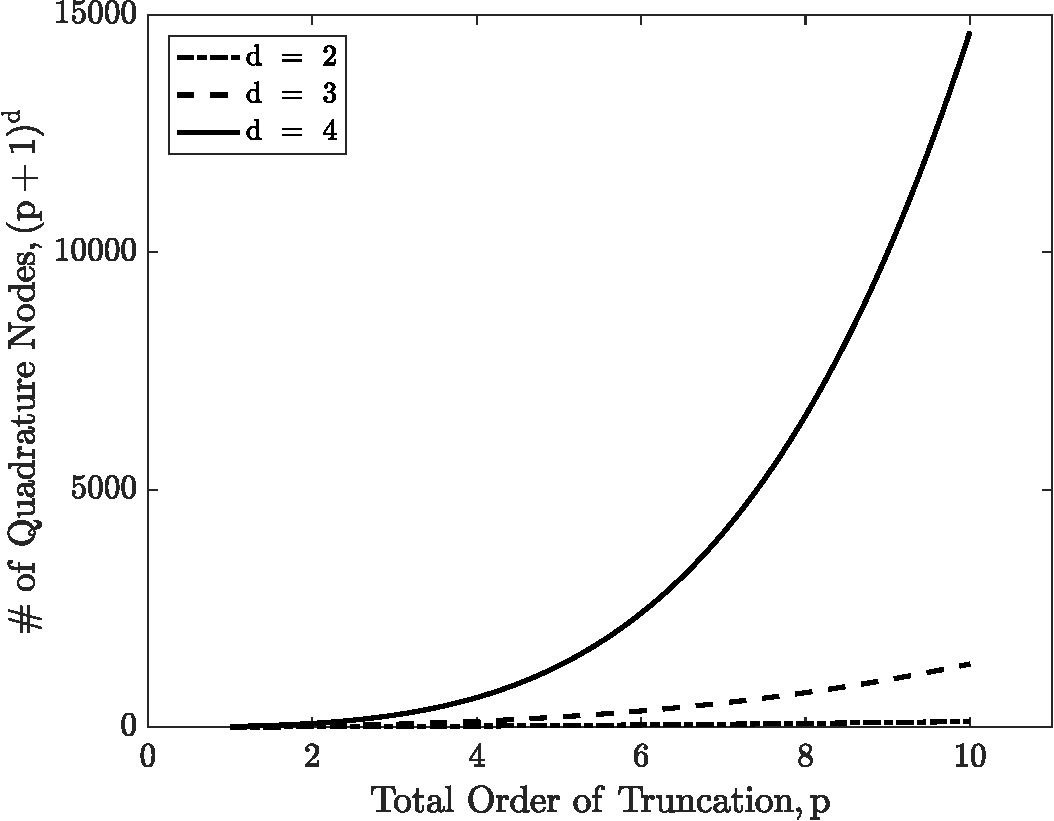
\includegraphics[width=0.70\textwidth]{./Figures/curse}
%\caption{Number of multi-dimensional Gauss quadrature nodes, $(p+1)^d$ is plotted against the PCE
% total order truncation, $p$ for 2, 3, and 4 dimensional polynomial basis functions.}
%\label{fig:curse}
%\end{center}
%\end{figure}




